\chapter{Sanskrit Letters}\label{chap:sktletters}

Like using the tool of Pāli letters, learning Sanskrit letters can be an enjoyable experience with this tool. You can open the window of Sanskrit Letters by menu Sanskrit > {\ppicons F}\ Letters. The window starts with Devanāgarī script, as shown in Figure \ref{fig:sanskrit-letters}. You can click a letter to see its classification, like you can do in the Pāli Letters. However, the arrangement of the grid is different, and the display of big letter is removed. Other functions are also similar. Please see Chapter \ref{chap:letters} for a refresh.

\begin{figure}[!hbt]
\centering
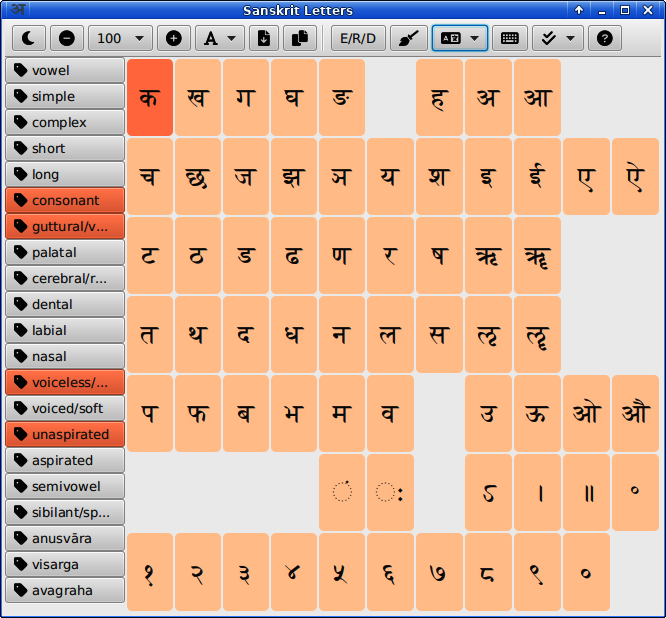
\includegraphics[width=0.9\linewidth]{images/sanskrit-letters.png}\\
\caption{Window of Sanskrit Letters}
\label{fig:sanskrit-letters}
\end{figure}

There are some symbols added to the grid, i.e., avagraha, single daṇḍa, double daṇḍa, and abbreviation sign. When you study Devanāgarī, you have to take these into consideration, particularly when you convert the script to Roman.

Hence, one function worth mentioning here is Roman transliteration. The tool can help you understand various ways of Roman conversion easier. When you convert the display script to Roman using {\faSix \symbol{"F1AB}} button, the default method can be selected by the option menu button (see Figure \ref{fig:sanskrit-letters-roman}). Note that the conversion is done directly from Devanāgarī. So, you will see `\pali{a}' ending in all consonants.

\begin{figure}[!hbt]
\centering
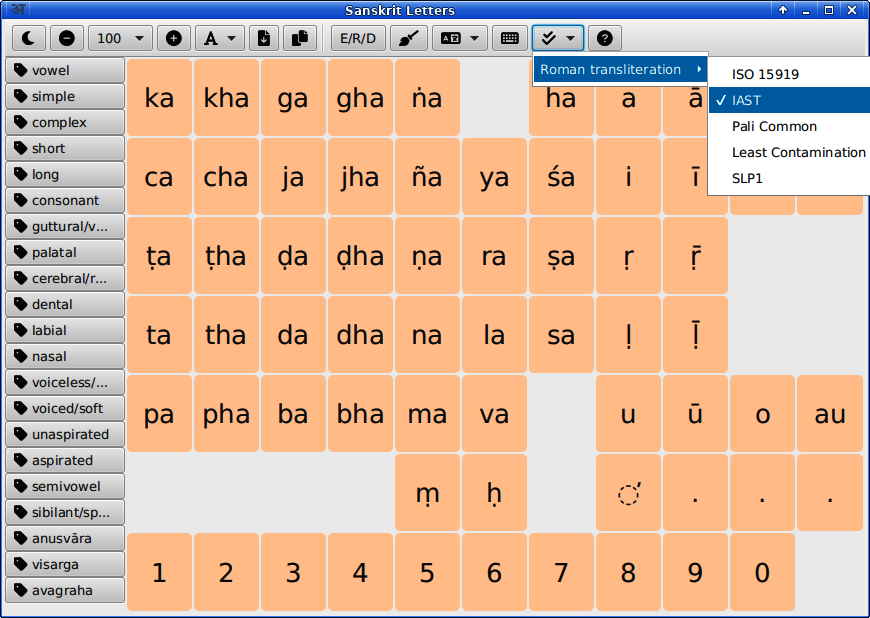
\includegraphics[width=0.9\linewidth]{images/sanskrit-letters-roman.png}\\
\caption{Roman transliteration in Sanskrit letters}
\label{fig:sanskrit-letters-roman}
\end{figure}

